\documentclass{ctexart}
\usepackage{amsmath} % 基本数学支持
\usepackage{amssymb} % 数学符号
\usepackage{framed} % 边框
\usepackage{graphicx} % 插入图片
\usepackage{float} % 图片H对齐环境
\usepackage{ulem}
\usepackage{cancel}
\usepackage{tcolorbox}
\tcbuselibrary{breakable}
\usepackage{enumitem}
\usepackage{color}
\usepackage{hyperref}
\usepackage{geometry} % 页面设置
\usepackage{subfigure} % 子图
\usepackage{listings} % 插入代码
\usepackage{threeparttable} % 插入三线表
\usepackage{fancyhdr}

\title{给果壳宝宝的数理基础课程学习经验指北}
\author{}
\date{\today}
\geometry{a4paper,left=2cm,right=2cm,top=1cm,bottom=2.5cm}

\pagestyle{fancy}
\fancyhf{}
\fancyfoot[C]{\thepage}
\renewcommand{\headrulewidth}{0pt}


\begin{document}

\setlength{\parindent}{2em}
\newtcolorbox{myexample}{breakable, arc = 0pt, outer arc = 0pt,
    colback = gray!5!white, colframe = gray!80!black,
    boxsep = 0pt, left = 10pt, right = 10pt, top = 10pt, bottom = 10pt,
    boxrule = 0pt, leftrule = 4pt, parbox=false}

\maketitle
\tableofcontents
\newpage
\section{自序:对意义的追问}
\vspace{0.5cm}
{\hfill \kaishu 人生到处知何似,应似飞鸿踏雪泥。——苏轼《和子由渑池怀旧》}
\vspace{0.5cm}

这样的文字,我想写已经很久了。在玉泉书院的朋辈辅导中心担任值班志愿者的经历,让我接触了许多不同专业的同学,他们往往带着各种对于数理基础课程的问题来(通常是课堂笔记或者作业),尽管我学识浅薄,但仍希望尽我所能去回答这些问题。当他们说着感谢推开门离开时,我总有些许愧疚感,我觉得我不配获得这些感谢——我其实并没有真正帮什么忙,且不说这些作业题我会不会,就算我真的不厌其烦地解释了每个细节,于他们又有多大帮助呢,毕竟这只是一道作业题。我知道在这些细碎的问题背后,藏着一些宏大的问题:学这些东西有什么用?为什么我很努力学了可就是学不会?我应该怎么学习?甚至,如果这些东西根本就没用,我应该花功夫学它们吗?

我一直在想这些问题应该如何回答,甚至有一个较为草率的提纲,还在一些场合分享过我的部分看法,可是一直没能动笔。一来考虑到我学识浅薄、思维狭窄,写出来的东西不一定有多大的意义,甚至还可能会带来误导;二是我总以“忙”为借口把这件事放下——“以后再写吧”,毕竟根据上面一点,即便写出来也很可能不能帮助很多人,那么写它于我就无关紧要了。

在我下决心写的那天(2025/2/13),心情很差,又陷入往常、老套的对自我意义的质问。看向正躺在坐垫上、已经陪伴了我13年的老猫,她正享受这一天中难得的清闲——狗睡觉了,没“人”来打扰她了。她的生活多么无忧无虑啊,可她的生命有什么意义呢?嗯……至少在陪伴我的13年里,她带给了我许多欢乐!虽然这是再小不过的一件事,毕竟我是谁呢?!可是于我而言,这是一件至大的事。

于是我想到,尽管我注定是一个彻彻底底的平庸的人,就像我的老猫,不能对这个世界带来任何一点的改变,但于我身边的、我能够帮助到的人,或许我的意义是重大的吧。想到这,我决定从进行了一上午的内耗中走出,打开电脑——去他的本科科研实践、去他的量子场论——开始动笔写下这些很早就想写的文字。如果这真的能够帮助到哪怕是一个人,那么于我而言,这简直是一件天大的事!

{\hfill 2025年2月13日\quad 于家中}

\section{前言}

在大一时,被国科大的学生提及最多的一个词大概就是“数理基础”。当然,这并不是因为它多么受欢迎,而恰恰因为它给予了同学们不同程度的困惑和精神上的折磨。这其中原因可以简单概括为:从高中浅层的套路化的理科学习到大学的数理基础课中存在巨大的鸿沟,导致同学们难以适应;而在尝试适应遭受打击时,逐渐产生了“灵魂之问”——学这玩意有啥用——进而产生了抵触的情绪,干脆糊弄一下得了,引发恶性循环。

这种课程衔接上的巨大鸿沟,其原因是多方面的。俄式教学模式下,在高中时学生就接触应用型的高等数学知识,进行了一定量的练习,得到了相应的思维能力的训练,并且(理想情况下)对于学科的严密性产生疑问,这时再接触分析学、代数学之类的学科就十分自然,这是符合历史发展也符合大多数人的认知模式的学习方式。但我国高中理科教育过于窄化,围绕着少得可怜的主题反复雕琢技巧,学生们接触不到更加丰富的知识,而解题的套路和技巧也都由经验丰富的教师归纳总结好并统一传授,训练思维能力的机会自然也就丧失了。在升入大学后,接触了大量全新的数学内容和思维方式(这些本应该是高中就简单接触的),自然会强烈不适应。况且国科大的数学教学模式一定程度上有些布尔巴基式,且普通物理的教学与大部分学校物理系的内容几乎无差别,这更加深了这条本就深得看不见底的鸿沟。

消除这条鸿沟显然是不现实的想法,在这篇文章中我想尝试去做的是提供一些(个人的)学习数理基础课程的经验,以期帮助更多同学顺利跨越这条鸿沟。这篇文章主要分为两个部分,第一部分试图回答数理基础课程有什么用,第二部分试图回答怎样学习数理基础课程,这两部分不是割裂的,在第一部分中实际上也包含了一些学习的建议。

最后我想说一点,如果读者您想在这篇文章中寻找“我应该怎样在最短的时间之内提高成绩”这类问题的答案,那么您实际上不用看我下面的长篇大论。因为据我所知,想要在短时间内提高成绩,最好的方法或许就是刷题和背题——尽量广泛地做题,把题目的套路记住并对不同类型的题目加以总结,在考试时遇到类似的题目就在脑中题库里搜寻先前做过的题目并且进行简单的变式应用——这就是我对这类问题的回答。可是,在这个过程中,除了(可能)获得了更高的分数,我们学到了什么呢?您当然可以谴责我太理想主义、不食人间烟火…… 我实际上已经被谴责过许多回了,可我仍想坚持我的初心,正如我在前面所说,我希望尝试触碰那些细碎的小问题背后的大问题。此外,我始终相信,大学教育的目标是“让人成为人”。果真如此,那么我们所学的数理基础,即便不像哲学、法学、文学那样能够直接对人生态度产生影响,但亦当增强我们的智慧、启蒙我们的理性。引港中文大学周保松教授的一句话作结:

\begin{quotation}
  \kaishu
  一门学问,如果能让你茶饭不思,教你辗转反侧,并改变你看世界看人生的方式,那它一定已走进你的生命。它不是你要应付的功课,不是无可无不可的一堆术语,而是成了你生命的真正关怀。(周保松《走进生命的学问》)
\end{quotation}

\noindent 我们能否让所学到的数理基础“走进生命”呢?

\section{学习数理基础课程有什么用?}
\vspace{0.5cm}
{\hfill \kaishu 山木,自寇也;膏火,自煎也。桂可食,故伐之;漆可用,故割之。人皆知有用之用,而莫知无用之用也。——《庄子·内篇·人间世》}
\vspace{0.5cm}

关于这个问题,最简单也最直白的回答是:没用!

实际上,对于大部分并不和数学、物理强相关的专业,国科大的数理基础课程,几乎是完全没用的。我们在两年的时间内学到的东西,不用说什么实数公理、西罗定理、约当标准形、洛伦兹变换、麦克斯韦方程组、原子光谱的精细结构…… 这些大家公认的抽象繁杂难懂的东西,就连积分的定义与运算、矩阵的特征值这类的看起来十分有用的东西,对于并不强相关的大部分领域,都并不常用。即便是真的有用,在使用时也几乎不用去在意那些无比抽象的证明——这正是令大多数同学感到无比头疼的部分。像很多人说的“学计算机/人工智能/…… 一定要学好数学”这类的话,在理解起来也要尤为注意,毕竟他们所谓的需要你学好的,和国科大的培养方案中所重点讲授的,存在一定的差别。就拿线性代数课程举例,由于使用的教材是科斯特利金的《代数学引论》,几乎所有班级的授课内容都紧密围绕代数学中的结构展开,并且重视证明而(几乎完全)轻视应用。在实际应用中异常重要的方法如矩阵分解(奇异值分解、极分解)并没有任何一个班级涉及,更不用提线性代数在当今的人工智能算法中的广泛应用了;用大量时间讲解若尔当标准形的存在性,甚至有的班级上升到了模的观点,却并没有说明为什么要研究若尔当标准形、在实际问题中若尔当标准形有什么应用;为大一新生讲解半个多学期的群、环、域的知识(据我所知甚至有的老师将这部分内容调整到了上半学期),并且几乎都是“定义-定理-证明”的讲解模式,没有什么例子和几何直观,即便举出一些例子,也因为同学们本身知识积累过少,而聊胜于无。

“吐槽”这么多,我是想说,从学到的知识这样一个“实”的角度来看,数理基础课是几乎没用的,但让我们从思维方式这样一个“虚”的角度来看一看。

\subsection{逻辑与结构}

数学和物理学是十分典型的具有严密的逻辑和结构的学科,其清晰的逻辑和精巧的结构可以算是现代科学体系中的所有学科的典范。在数理基础课中训练的逻辑思维,对于学习其他学科会起到很大的帮助。

大学课程对逻辑与结构的强调,与高中学习存在很大的不同。在高中时,我们关心的通常是:这个题有什么技巧或者套路。受到这样的思维定式的影响,许多同学在学习大学的课程时也将关注重心放在的解题上,并没有学到一门学科的框架和核心思维方式,也导致对逻辑思维训练的欠缺。这就经常导致这样的问题:证明这个定理的目的是什么?引入这个概念的目的是什么?这种问题问的是“动机”(motivation),当我们对一门课程的结构和逻辑十分清楚时,很多这样的问题就自然解决了。


\begin{myexample}
  以线性代数中线性算子理论为例。

  翻开《基础代数(第二卷)》的目录,第二章线性算子包含五个小节:“向量空间的线性映射”,“线性算子代数”,“不变子空间和特征向量”,“商算子和对偶算子”,“约当标准形”

  我们为什么要研究线性映射,因为它将实际问题中的许多不同的变换都抽象出来,又保留了线性这一核心性质。抽象是数学的核心,它能够使得我们用同一套语言研究截然不同的东西,而更重要的是,在抽象的过程中我们扔掉大多数东西而保留少部分特质,这导致问题的关键被突出强调出来,有助于解决问题(波利亚将这种现象称为创造者悖论:越宏大的目标越有机会成功)。

  研究复杂的变换通常将其拆分为简单的部分,这就导致我们研究变换的复合(乘法)和叠加(加法)。由于作用的空间不同,变换的复合存在一定限制,最理想的情况就是线性算子$\mathcal{A}: V \rightarrow V$.这种情况下线性算子间的组合构成代数——这又是一层抽象,我们忘掉线性算子本身作用在什么上,只考虑它们之间复合和叠加的结果。\textbf{在线性代数的学习过程中应经常注意无处不在的抽象过程!}

  研究一般的线性算子的一个核心问题就是搞清楚一个线性算子$\mathcal{A}$作用于任何一个向量$\mathbf{v}$上的产生的后果,为什么要研究这样的问题呢?因为有许多实际问题都可以用线性算子建模为下面的方程:
  \begin{center}
    $\mathbf{x}(t + 1) = \mathcal{A}\mathbf{x}(t)$(离散) 或 $\dot{\mathbf{x}}(t\mathcal{) = A}\mathbf{x}(t)$(连续)
  \end{center}

  我们希望关注这样的系统的时间演化行为,这就要求我们研究算子$\mathcal{A}$对向量的作用。基本的研究方法就是先寻找一些简单的情况,在通过线性讲一般情况分解为简单情况的叠加——这就自然地导致特征值、特征向量、不变子空间概念的引入。在代数学中,伴随子结构出现的往往有商结构,这是因为我们希望能够将“一块大蛋糕”分成许多层,如果能够研究清楚每一层的样子和不同层间的关系,便可以看清整个“大蛋糕”。这是十分“代数”的思维方式,\textbf{在学习中也应多多体会总结代数学中的思维方式}。为了解决整个问题,我们还应该考虑如何将一般的情况化为简单的情况,因此要考虑不同的特征向量的关系——可对角化的研究。在无法对角化的情况,作为弥补,引入广义特征向量——这导致约当标准形的研究。回顾这样一整套思路下来,最核心的概念就是线性,因为线性我们才可以将复杂的情况写为简单的情况的叠加,那么我们是否可以思考,对于非线性的情况应当怎样处理?\textbf{在完成一整个体系时,应当回到最初,看看哪些假设是关键的,如果扔掉这些假设还可以进行吗?}

  这样一看,这一整章的思路是不是很清晰!
\end{myexample}


上面所说的这些不仅应用于大方面,即一个学科、一章内容,还适用于小方面,即一个定理或问题。高中数学的解题步骤往往较为简短,即便是压轴题有很长的步骤也都是较为直接的计算,但大学课程中的许多证明往往很长,初学时容易迷惑,这就是因为对证明的结构(也就是常说的big picture)没有清晰的认识。正确的方法是,先理清楚每一部分是在做什么(如果并不在意细节,这时就可以结束了),理解证明的整体结构,再深入每一部分仔细研究。

尽管我这里说的一切都局限在数理基础课中,但容易看到,这种思维方式在学习任何一门课程、阅读任何学术论文乃至阅读互联网上的文章时,都发挥作用。科学发现永远不是凭空冒出来的,相比于被动接受各种事实,勤于问“为什么这样想”(例如:这个实验为什么这样设计,其关键突破在哪里?)、“整个流程的逻辑是什么,是否遵循什么基本原则”、“这个领域的核心框架是什么”(例如:中心法则实际上包括了分子生物学的核心问题)这样的问题,对于我们的学习有很大的帮助。

\subsection{解决问题的方法}

在数学、物理学中,包含着几千年来许多人类顶尖的头脑思考、解决问题的方式。物理学中以第一性原理出发的思考方式,启发着许多学科的发展。此外,通过构建数学模型以定性或定量解释问题的方式也出现在其他学科中,并且在近年来越发热门。



\begin{myexample}
这里举出生物学中的一些例子:
\begin{enumerate}[leftmargin=*, labelsep=0.5em]
\item 图灵斑图(Turing Pattern):图灵斑图是图灵在1952年试图解释自然界中规律性班图的形成机制的理论,在这种理论中,激活剂和抑制剂以不同的速度扩散,相互制衡,导致结构形成。这样的系统可以用简单的偏微分方程描述,并且给出定量的预测。尽管图灵在提出这一理论后不久逝世,而这一理论也沉寂了许久,但随着分子生物学技术的发展,在许多生命系统中,图灵所预期的激活剂和抑制剂被发现,并且当人为减少或增加这些化学物质的活性时,形态的变化符合方程的预期。这是典型的理论引领发现的例子。
\item 霍奇金-赫胥黎模型(Hodgkin-Huxley model):这个方程以及其背后的大量实验验证,帮助两人获得了1963年的诺贝尔生理学与医学奖。它仅用简单的电学模型就十分准确地给出对神经脉冲的定量预言,并且还前瞻性地预测了通道蛋白的结构和开放、关闭动力学。
\end{enumerate}
\end{myexample}


波利亚(Polya)在他的著作《怎样解题》(这是一部十分值得阅读的作品!)的序言中写过这样一段话:

\begin{quotation}
  \kaishu
  虽然本书特别关注对于数学专业的学生和教师的要求,但它也应能引起任何关心创造和发现的各种途径和方法的人的兴趣…… 在解答这道或那道不涉及物质利益的题目的愿望背后,也许有着一个更深切的好奇心,一个要求理解解答的各种途径和方法、动机和步骤的愿望。
\end{quotation}

学习数理基础课程,解决难题的目的不在于其本身,而在于从中寻找解决更广泛问题的思维方式,而这实际上对于从事其他的创造发现工作都有帮助。就我而言,当我面对一个生活中一个复杂的决策或完成一个任务时,我会有意识或无意识地考虑,有没有什么最基本的原则、这个任务本质想达成什么样的目标。有了这些作为立足点就不会被一些表面上的困境所阻碍。这种关注第一性原理的思维方式或许就源于物理学的训练。

\section{应该怎样学习数理基础课程}

究竟怎样学习数理基础课?经过高中三年的磨练,先想到的肯定是刷题。这时就会听到一些声音:“别刷你那题啦,那是高中的学习方式!”否定当然十分简单,但当我们去寻找属于大学的学习方式的时候,似乎又不再能听到什么建议。毕竟怎样学习、怎样思考是一个颇为抽象的事,不容易言说。所以我也不打算去尝试说那不可说之物,即便真的做到了也会使给出的建议抽象难懂,相反,我想以对一系列小问题的回答作为我对“怎样学习数理基础课程”这样一个大问题进行解答的尝试。为了避免回答过于抽象,我结合了一些例子,考虑到大一同学的知识水平,我尽量将例子限制在大一基础课的范围之内。

接下来我所写的远非原创,在网络上和一些书籍种能够找到许多类似的说法,尽管我并没有对这些说法进行简单的搬运,但我必须承认我的学习方法和思维方式实际上很大程度上受到了已有的这些说法的影响,以至于我所输出的建议几乎可以看作对它们的简单复制。不过我认为将其汇总并写出仍然是有意义的,因为可悲的是,现在许多(即便是一流大学的)大学生并不具备基本的搜索、查阅资料的能力,我在这里权当授人以鱼了。

\addcontentsline{toc}{subsection}{问题一:数学课程中的概念和证明太抽象理解起来困难有什么应对方法?}

\noindent$\blacktriangleright$\;\textbf{Q1:} 数学课程中的概念和证明太\textbf{抽象}理解起来困难有什么应对方法?

\noindent$\blacktriangleright$\;\textbf{A1:} 

除了极少数天才能够完全习惯于纯粹的抽象思维,大多数人都需要不同的方法来应对并逐渐接受抽象思维。

\begin{myexample}
  举我自己的一个例子,我第一次接触数学分析是在高一的时候,在假期里用中科大的《数学分析教程(上册)》自学数学分析,但学到数列的上极限和下极限就卡住了。书上写:
  
  \begin{quote}
    我们把数列$\{ a_{n}\}$的收敛子列$\{ a_{k_{n}}\}$的极限称为$\{ a_{n}\}$的一个极限点,设$E$是由$\{ a_{n}\}$的全部极限点构成的集合,则$a^{*} = \sup E,\ a_{*} = \inf E$分别称为$\{ a_{n}\}$的上极限和下极限.
  \end{quote}
  
  这个定义在当时就把我难住了,又是收敛子列又是上确界下确界,这么多概念,到底在说啥?当时的我看书时只是关注书上的文字,关注每个概念的定理的陈述。对我来说,上确界就是“上确界”,也就是书上的定义:
  
  \begin{quote}
    设$E$为一非空的上有界的集合,实数$\beta$满足(1)对任何$x \in E$有$x \leq \beta$,(2)对任何$\epsilon > 0$存在$x_{\epsilon} \in E$使得$x_{\epsilon} > \beta - \epsilon$.则称$\beta$为集合$E$的上确界,记为$\beta = \sup E.$
  \end{quote}
  
  但当时在我脑中,关于上确界究竟在说一件什么事,并没有直观的认知,因此自然看到上极限的定义就开始迷糊。
  
  书上简单举了一个例子之后,立刻又开始证明了一系列定理:
  
  \begin{quote}
    \begin{enumerate}[leftmargin=*, labelsep=0.5em]
    \item $a^{*} \in E$
    \item 若$x > a^{*}$则存在$N \in \mathbb{N}^{*}$使得当$n \geq N$时有$a_{n} < x$
    \item 若存在$N \in \mathbb{N}^{*}$使得当$n > N$时有$a_{n} \leq b_{n}$则:$\liminf\limits_{n \rightarrow \infty} a_{n} \leq \limsup\limits_{n \rightarrow \infty} b_{n}$
    \item $\lim\limits_{n \rightarrow \infty\ }{\inf_{k \geq n}a_{k}} = \liminf\limits_{n \rightarrow \infty}a_{n}$
  \end{enumerate}
  \end{quote}
  
  这些定理的证明在我当时看来也是异常得抽象,于是我的第一次数学分析学习就在此结束了。
  
  可当我高考结束后再次拿起这本书,再次从头开始看,看到这里就发现原来一切都是如此显然。上确界简而言之就是“最小的上界”——它是上界,但再小一点就不是了。我可以想象一幅画面:在数轴上散布着一堆点,它们是集合$E$的元素,你在数轴上画了一条线,站在这条线上,你能看到数轴上的这些点在向你接近,但无论如何就是无法超过你的位置(见下图)——有一种“在悬崖边上跳舞”的感觉(\url{https://www.bilibili.com/video/BV1Df4y1j7jP})。有了这些直观,上确界的定义也就十分显然了:数轴上的点永远无法超过你,这就是$\forall x \in E:x \leq \beta$.
  但你“在悬崖边上跳舞”,任何一点风吹草动就会“坠入深渊”,这就是$\forall\epsilon > 0\ :\exists x_{\epsilon} \in E\ s.t.\ x_{\epsilon} > \beta$.
  
  \begin{figure}[H]
    \centering
    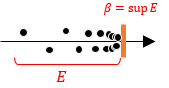
\includegraphics[width=.22\linewidth]{fig/上确界.png}
    \caption{上确界示意图}
    \label{fig:sup}
  \end{figure}
  
  理解了上确界,上极限也就不难理解了。数列和数的集合很像,都是数轴上的一些点,只不过这里有增加了一个新的维度——时间,也就是下标$n$.
  你可以想象站在数轴上你画的线外,看着另一个人一个接一个地将数列中的项点在数轴上。这些点时而靠近你、时而远离你,即便经过了很长时间仍然摇摆不定。这时我们扔掉数列中的一些点,剩下的点有了统一的趋势(这就是取$\{ a_{n}\}$的子列$\{ a_{k_{n}}\}$),你看到有些时候,剩下的这些点慢慢停在离你有一定距离的地方,有些时候(取决于你扔掉哪些点,也就是取什么样的子列)剩下的点慢慢停在了离你非常近的位置,但仍然无法超过你,那么你就站在数列的上极限上(见下图),对于下极限也能同样思考。
  
  \begin{figure}[H]
    \centering
    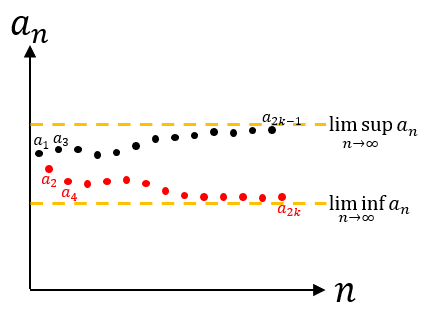
\includegraphics[width=.45\linewidth]{fig/上极限.png}
    \caption{上下极限示意图}
    \label{fig:limsup}
  \end{figure}
  
  如果你对着这张图,以及一些其他的例子看一段时间,结合定义,就不难发现,直观地说,在下标非常大时,数列中的项几乎就在上下极限间来回摆动——它们当然可以超过上极限或者下极限(尝试找到一个例子画一张图),但当下标非常大时,数列中的项不会超过上极限太多也不会低于下极限太多。某种程度上,上下极限就像是为数列设置了一个无形的屏障。当然,如果你十分严谨,立刻就会意识到我上面说的这一切纯属胡扯,但是你一定也会承认,这些直观的语言,能够为我们带来许多见解。比如,现在回看上面我列出的四个命题,有些是不是变得十分显然?
\end{myexample}
  
  总结一下,为了理解一些抽象的概念和证明,应当做到:
  
\begin{enumerate}[leftmargin=*, labelsep=0.5em]
\item 对\textbf{基本概念}掌握熟练并形成\textbf{直觉}:正如我在前面所说,数学是一个逻辑十分严密的庞大的“建筑”,每一个新的概念都依赖于旧的概念,而定理的证明也都十分依赖基本的概念和一些简单的性质。就像我在上面所举出的例子,为了理解上极限,应当对上确界及其性质十分熟悉,我在第一次学习数学分析时,对上确界只是一知半懂就开始学习上极限,看不下去是自然的了。

根据我的观察,许多同学说自己不会做题、看不懂一个证明,并不是因为不具有一定的数学思维方法,而是连题目或证明中涉及到的基本概念都不清楚!这实际上就受到了高中的学习方式的影响——高中数学的内容很少,涉及到的概念不多并且都十分直观很快就能接受,因此许多同学养成了下课即做题的习惯。但在大学里,很多时候一节课就要介绍五六个新概念,并且都较为抽象,许多同学下了课立马对着作业开始进行一番苦思随即发现不会做。且不说这时你是否已经将概念内化,变成一种直觉,实际上就连这些概念是什么你都需要回去翻笔记,相关的定理更是完全不知道,那么你怎么可能做出题呢?(如果你发现有这种情况,那么就应该停下来不要再尝试做题了,把笔记或书本再看一遍,尤其关注那些不熟悉的概念和定理)

因此,在学习中,\textbf{对于每个概念都应该十分熟悉,能够清楚地说出它的定义是什么?有什么相关的重要的性质}(通常是书上紧随着一个概念出现的几个定理,\textbf{对于这些定理的陈述应当十分熟悉,最好能够也对其证明有一定的熟悉度},因为这些证明中往往包含了运用这个概念的基本方法)?我的建议是,\textbf{在学完一节课准备做题之前,试着把书合上,能不能在纸上写出这节课讲了什么概念,与这些概念相关的定理是什么,有什么典型的例子?}但这还不够,陶哲轩(Terence
Tao)曾经说过,在数学学习和研究中,有三个阶段——前严谨阶段、严谨阶段和后严谨阶段。如果我们能够熟悉概念和相关的性质的表述,那仅仅走到了“严谨阶段”,接下来应当将这些概念和性质内化为一种直觉。具体来说,\textbf{你能不能用短且直观的一句话将一个很长的定理在说什么事概括出来?能不能将一个概念和一个图像联系起来?}这种概括一定不是十分精确严格,但你应当知道为了使得其严格化应当诉诸什么定理。比如我在上面说,“在下标非常大时,数列中的项几乎就在上下极限间来回摆动”,这句话就直观但不严格,什么是“非常大”,什么是“几乎”?但我知道怎样严格地表述出来:我们知道对于任何$x > \limsup a_{n}$,都能够找到$N \in \mathbb{N}^{*}$使得当$n > N$时有$a_{n} < x$. 这就将“几乎”和“十分大”严格地说了出来。人的推理是十分依赖于直观的,很少有数学家能够完全对着抽象概念进行推理,大部分人的推理方式都是先借助一个一个的直觉看到结果,再慢慢补全严格的证明。

\item 多考虑一些例子:当你对一个概念迷惑时,找到或者构造一个例子,越具体越好,对着这个例子思考概念,\textbf{这个概念的表述在你找到的例子中怎样体现?}在学习数学和物理学时,例子是异常重要的!\textbf{尽量做到对每个比较复杂的概念、定理、公式,都能在脑中熟记一个例子。}这些例子甚至不必是数学的,例如曾经有同学说无法理解商映射和映射的典范分解,《代数学引论》中是这样写的:

\begin{quote}
集合$X$对应于等价关系$\sim$的划分记为$X/\sim\ $,称之为$X$关于$\sim$的商集.
映射$p:x \mapsto p(x) = \widetilde{x}$称为$X$到商集$X/\sim$的典范投影.
映射$f:X \rightarrow Y$给出$X$上的等价关系$\omega_{f}$,定义为:$\forall x,x^{'} \in X:x\ \omega_{f}\ x^{'}\  \Leftrightarrow f(x) = f\left( x^{'} \right)$.
该等价关系诱导出商映射$\overline{f}:X/\omega_{f} \rightarrow Y$,由法则$\overline{f} \cdot p(x) = f(x)$给出,此处$p$是$\omega_{f}$对应的典范投影.
分解式$f = \overline{f} \cdot p$称为映射$f$的典范分解.
\end{quote}

于是我给出了这样一个例子:假设总共有两个任务,你要分配给五个人。集合$X = \{ 1,2,3,4,5\}$表示这五个人,$Y = \{ a,b\}$表示两个任务,映射$f$把每个人对应到两个任务中的一个.
由于直接分配过于复杂,你先将五个人分为两组$\{ I,II\}$,分组的标准是将你想分配同一个任务的人分到一组.
即$X/\omega_{f} = \{ I,II\}$(严格来说这里不正确,只能说在相差一个同构的意义下相等,即$X/\omega_{f} \simeq \{ I,II\}$,但对初学者来说,为了避免更进一步的抽象,这个差别可以暂时忽略),典范投影$p:X \rightarrow \{ I,II\}$将每个人对应到其所在的组.
现在你只需要为每个组分配任务,这就是$\overline{f}:\left\{ I,II \right\} \rightarrow \{ a,b\}$.假设现在想知道某个人$x$对应的任务$f(x)$,首先找到它所在的组$p(x)$,在找出这个组被分配的任务$\overline{f}(p(x))$即可,这就是典范分解.

此外,不仅对于理解一个概念,在学习一个证明时,例子也非常重要。这包含许多方面:首先,找到一个符合定理的条件的例子,观察这个定理是如何在这个例子上发挥作用的可以帮助理解定理的直观含义;其次,构造一个反例,例如定理说在满足P时有Q成立,那么构造一个P不满足时Q不成立的例子(这种例子的构造是有挑战性的,仅仅让Q不成立很容易,但\textbf{能不能让你的例子达成尽量接近Q的结果?}),或者尝试构造一个在P成立时Q不成立的例子,这显然构造不出来,但尝试的过程能够帮我们认识到这个定理为什么应当成立。

\item 借助几何直观:多画一些示意图,就如在上面画的两张图那样,能够让自己更快理解。
\item 保持逻辑清晰:很多同学说一个证明或某一章的内容太抽象,往往是因为它很长,看一会儿就绕晕了。这个时候拿出笔在书的旁边写上:\textbf{现在我要做什么?我已经知道了什么结果?(这可以通过先忽略细节,粗略看一遍实现)我还需要证明什么就可以得出结论?有什么相关的定理可以帮我完成证明?}这能够很好地帮助我们理清思路。
\end{enumerate}

\addcontentsline{toc}{subsection}{问题二:怎样阅读数学、物理类的教科书?}
\noindent$\blacktriangleright$\;\textbf{Q2:} 怎样\textbf{阅读}数学、物理类的教科书?

\noindent$\blacktriangleright$\;\textbf{A2:}

关于怎样阅读数学书籍,其实在对第一个问题的回答时已经说了许多了,这里就只提及哈尔莫斯(Paul
Halmos)的一段十分著名的阐述:

\begin{quotation}
  \rmfamily Don't just read it; fight it! Ask your own questions, look for your own examples, discover your own proofs. Is the hypothesis necessary? Is the converse true? What happens in the classical special case? What about the degenerate cases? Where does the proof use the hypothesis?
\end{quotation}

\begin{figure}[H]
  \centering
  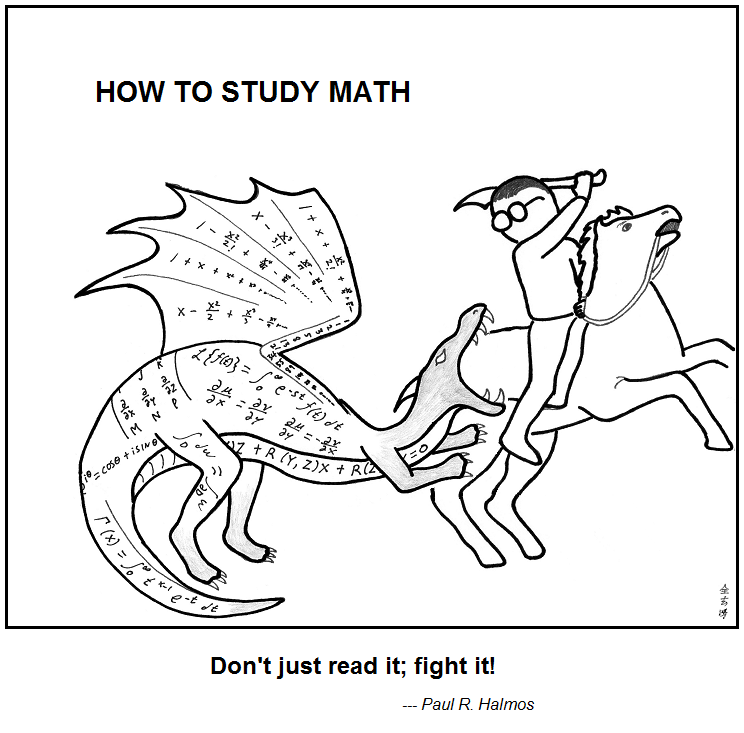
\includegraphics[width=.5\linewidth]{fig/Halmos.png}
  \caption{Don't just read it; fight it!}
  \label{fig:halmos}
\end{figure}

在哈尔莫斯的阐述中,蕴含了许多读书时的技巧:

\begin{itemize}
\item Is the hypothesis necessary?——考虑定理的条件是否是必要的,如果没有这个条件定理是否能够成立?考虑这种问题能够帮助我们理解某个条件对定理的重要性,这通常能够帮助我们找到对于定理的证明。与之相关的是最后一条Where does the proof use the hypothesis?——定理在证明时哪里用到了该条件,这种使用该条件的方法是你熟知的吗?如果你熟知,那么你能否说出为什么作者要这样用?如果你来写这个证明能想到吗?如果你不熟知,那么是否可以将这种使用条件的方法进行推广,放到你自己的“工具箱”中?
\item What happens in the classical special case? What about the degenerate cases? —— 该技巧是关于如何考虑例子的。在一些已知的特殊情况下,能否验证定理成立?在一些退化情况(即某些条件被十分平凡地满足)下,能够验证定理成立?这些情况能够建立对于定理的直觉,也能帮助我们想到对于定理的证明。
\end{itemize}

\textcolor{red}{【未完】}

\addcontentsline{toc}{subsection}{问题三:看答案都能看懂,但自己无法独立解答怎么办?怎样想到解题思路?}
\noindent$\blacktriangleright$\;\textbf{Q3:} 看答案都能看懂,但自己无法独立解答怎么办?怎样想到\textbf{解题思路}?

\noindent$\blacktriangleright$\;\textbf{A3:}

波利亚在《怎样解题》中给出了这样的总结:

\begin{figure}[htbp]
  \centering
  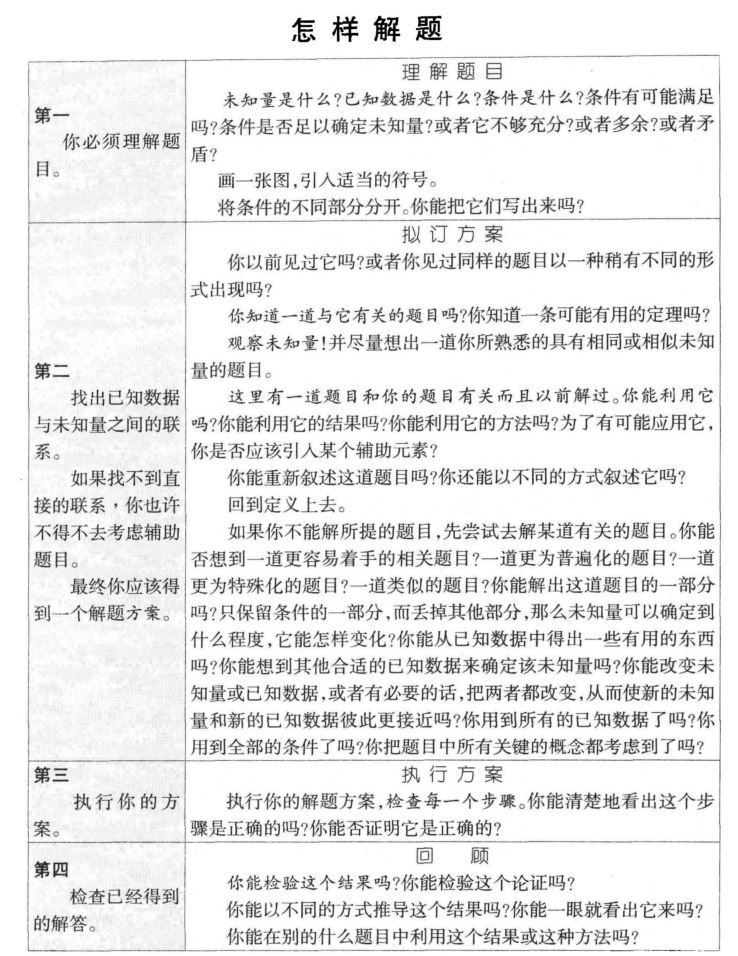
\includegraphics[width=.9\linewidth]{fig/怎样解题.JPG}
  \caption{怎样解题}
  \label{fig:polya}
\end{figure}

关于例子,这本书中有许多生动的阐述,但涉及的题目都较为初等。类似但更加详细的阐述可见陶哲轩的作品\textit{Solving Mathematical Problems: A Personal Perspective}(中文翻译由人民邮电出版社出版,名为《陶哲轩教你学数学》),从中可以看到当今世界最天才的数学家是如何解决数学竞赛问题的。强烈建议阅读这本书的第一章“解题的策略”(\url{https://www.ituring.com.cn/book/tupubarticle/22734})



\begin{myexample}
  下面举出几个例子:
  \begin{enumerate}[leftmargin=*, labelsep=0.5em]
    \item 一个数学分析中的问题
    \item 一个线性代数中的问题\textcolor{red}{【未完。暂时找不到难度不太低同时又能清晰地阐述各种思考问题的方法的问题】}
    \item 一个物理问题(这应该是哪一本书中的习题,但我并不记得在哪里了,只对题目有印象):
    
    一个半径为$a$的球形电极被深埋(深度$h \gg a$)在大地中,假设大地是均匀的导电介质,电导率为$\sigma$,介电常数为$\epsilon$.
    向电极通入电流$I$,在电流达到稳恒状态后,求:(1)电极表面的自由电荷密度(2)大地中的自由电荷密度和电流分布(3)根据欧姆定律计算热功率
    
    \begin{figure}[H]
      \centering
      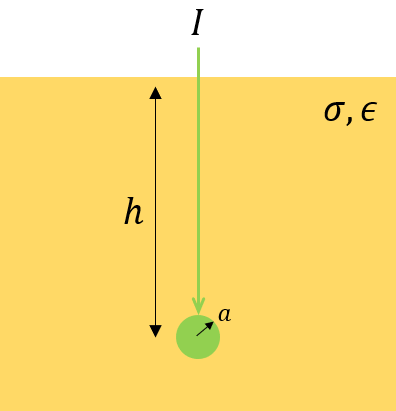
\includegraphics[width=.25\linewidth]{fig/大地电流.png}
      \caption{球体电极问题示意图}
      \label{fig:electrode}
    \end{figure}
    
    这个问题不算困难,但却很容易能难住许多同学。这是因为它涉及的情景与大家较为熟知的、十分简单明了的电路不同。那些涉及电路的问题,尽管计算十分复杂,但往往比较直接而且套路化。但这样的问题模型并不直接,许多同学看一眼没有思路就放弃了。面对这种并不套路化的问题,应该如何思考?——\textbf{应该抓住最根本的物理原理,根据题目条件将我们一定能够确定的东西写下来,一点一点分析最终得到答案,不能期待直接就看透题目的解法。}
    
    面对这个问题,我们知道哪些永远对的基本原理?
    
    \begin{itemize}
      \item 题目涉及电流,肯定需要使用微分形式的欧姆定律$\mathbf{J} = \sigma\mathbf{E}$\textbf{.}
      \item 关于静电场的问题一定需要静电场的高斯定理$\nabla \cdot \mathbf{E} = \frac{\rho}{\epsilon_{0}}$.
      \item 题目提到“稳恒电流”条件,它的微分形式为$\nabla \cdot \mathbf{J} = 0$.但这并不足够,它只给出了介质中电流的稳恒条件,还有外界输入的电流$I$,它输入到电极上并由电极流到大地中,这过程中电极上不会随时间积累电荷,因此有$I = \iint_{S}^{}{\mathbf{J} \cdot \mathbf{n}\ dS}$其中积分是对球体的表面进行的。
      \item 题目涉及电介质,那么就还有电位移与电场强度的关系$\mathbf{D} = \epsilon\mathbf{E}$,以及相应的高斯定理$\nabla \cdot \mathbf{D} = \rho_{f}$.
      \item 题目特别关注球体表面的自由电荷分布,因此肯定涉及边值关系$D_{2n} - D_{1n} = \sigma_{f}$.
      \item 题目还给出的一个假设$h \gg a$,这意味着可以忽略大地表面的影响,电极就像被放在一个填满整个空间的均匀介质中一样,因此我们知道电极附近的电场和电流分布一定是球对称的。
      \item 题目提到欧姆定律,即$P = I^{2}R$,这意味着我们需要计算电阻$R$,它与电阻率的联系是$R = \frac{L}{\sigma S}$.
    \end{itemize}
    
    这其中的每一步都是很基本的物理知识,单独拿出来肯定绝大部分同学都能意识到。(如果面对这样的问题,你不能做到对着题目的条件至少把所有可能和求解该问题相关的公式都列出来,那就说明你对一门课的基础知识掌握还欠缺!)\textbf{面对一时没有思路的问题时,先拿出一张纸,边阅读题目边尽可能多地列举与这个问题相关的事实,接着看看这些事实如何组合得到新的事实并将它们写下来}(如果不写下来,很可能经过了复杂的推演之后就忘记了)\textbf{,在这个过程中还应始终注意我们需要求出什么}(最好也将它写在纸上)\textbf{,正向推理与反向推理结合,如此往复,很可能就足够解决这一问题了!}很多同学遇到不会的题的时候往往会“骗分”把所有相关的公式列上,但实际上当我们把公式列出来了,知道公式里面的量代表什么物理意义时,只要耐心分析一点点推进,题目也基本上就完成了。
    
    首先看到,我们有$\nabla \cdot \mathbf{J} = 0,\mathbf{J} = \sigma\mathbf{E},\nabla \cdot \mathbf{E} = \frac{\rho}{\epsilon_{0}}$,这三个联合起来给我们了$\nabla \cdot \mathbf{E} = 0 \rightarrow \rho = 0$,这似乎不能回答第二问,不过再看到我们有的$\mathbf{D} = \epsilon\mathbf{E,}\nabla \cdot \mathbf{D} = \rho_{f}$,结合上面就立马给出了$\rho_{f} = 0$.
    
    对于第一问,我们关注电极表面的问题,上面列表里有关的公式是$I = \iint_{S}^{}{\mathbf{J} \cdot \mathbf{n}\ dS}$.由于我们知道电极附近电流(电场)分布均匀,就有$I = 4\pi a^{2}J \Longrightarrow \mathbf{J} = \frac{I}{4\pi a^{2}}\mathbf{e}_{\mathbf{r}}$.再看看目标,我们希望求表面自由电荷,与之相关的公式就是边值关系,也就要知道$\mathbf{D}$,可是$\mathbf{D} = \epsilon\mathbf{E}$.因此只要知道$\mathbf{E}$.再看看列表里的公式,有了$\mathbf{J}$就可以知道$\mathbf{E}\mathbf{=}\frac{\mathbf{J}}{\sigma}$.嗯,我们离胜利不远了(剩下的问题交给读者吧!)
  \end{enumerate}
\end{myexample}

\addcontentsline{toc}{subsection}{问题四:许多老师强调学物理要重视物理图像,什么是物理图像?怎样重视物理图像?}
\noindent$\blacktriangleright$\;\textbf{Q4:} 许多老师强调学物理要重视\textbf{物理图像},什么是物理图像?怎样重视物理图像?

\noindent$\blacktriangleright$\;\textbf{A4:}

简而言之,重视物理图像就是锻炼把数学公式和物理意义联系起来的能力,从最字面意义上理解,它关注的是这样一个问题:我写下了一个表达式,它整体对应于什么\textbf{物理过程}(能否在脑中“播放一个动画”),每一项对应于哪个子过程,其中的\textbf{每一个字母都是什么含义}(能否画一个图标出来)?

更进一步地,知道了表达式对应的物理过程,可以问这些问题:

\begin{itemize}
\item 我能不能不进行复杂的计算就\textbf{猜出答案大概是什么样子的}?
\item 我计算出了一个结果,\textbf{能否说明它应该是对的(justify your result)},比如这里的正负号是否正确、正比或反比关系是否合理。做到这点除了要明确物理过程之外,还通常要借助一些物理思维,如考虑\textbf{比较容易通过物理直觉感知到的特殊情况}、\textbf{不同物理现象的类比}、\textbf{量纲分析}等。
\end{itemize}



\begin{myexample}
  对于上面提到的几点,下面举出几个例子:
  \begin{enumerate}[leftmargin=*, labelsep=0.5em]
    \item 对热力学第一定律的理解:$\Delta E = W + Q$.这一点学过高中物理的同学都能背过,但是在最开始使用时都会出错,尤其是在过程复杂时。式中$\Delta E$是考虑的系统的能量增加量$\Delta E = E_{f} - E_{i}$,$W$是给定的过程中外界对系统做功而$Q$是给定过程中系统从外界吸收的热量。在使用该公式时,关键是要明确研究的热力学系统是什么(相应地外界是什么),$W$与$Q$是正是负(这里不用死记硬背,考虑特殊情况,如果系统与外界绝热则$\Delta E = W$,当外界对系统做功则向系统输入能量,系统能量增加$\Delta E > 0$,因此$W > 0$.类似考虑$Q$的正负。上面的论证可能很平凡,但其背后的思想是普遍的——当我希望知道某些量的性质时,我考虑了一个虚构的、尽可能简单的系统和过程,通过对这个过程的分析得出结论,获得对这个物理量的物理直觉)。在实际应用该方程时,就像上面说的,\textbf{画几幅图标出各个物理量}(如用箭头标明正负),写下方程时不能仅仅看着数字要\textbf{回顾数字代表了什么}(用自然语言把数字解释一遍),这在最开始很耗费时间,但能够大大提高正确率。
    
    \item 变质量物体的运动方程(密歇尔斯基方程):$\mathbf{F} = m\frac{d\ \mathbf{v}}{d\ t} + \left( \mathbf{v} - \mathbf{v}^{'} \right)\frac{dm}{dt}$,有时会引入分离速度$\mathbf{u} = \mathbf{v}^{'} - \mathbf{v}$而将方程写为$\mathbf{F} = m\frac{d\ \mathbf{v}}{d\ t} - \mathbf{u}\frac{dm}{dt}$,教科书上还会提到在$\mathbf{v}^{'} = 0$的特例$\mathbf{F} = \frac{d}{dt}(m\mathbf{v})$.看到这么多公式,可能有些同学就要开始背诵了,但且慢,对于一个公式,最重要的是要明确:
    
    \begin{enumerate}[leftmargin=*, labelsep=0.5em]
      \item 这个公式描述了什么\textbf{物理过程}?它的\textbf{适用范围}是什么,是普适的还是对某些特殊情况成立?公式里的\textbf{每一项的含义}是什么?
      
      \item 这个公式是\textbf{如何推导出来}的?
      
      \item 这个公式\textbf{为什么应该是对的}?不进行推导能不能给出它可能成立的证据?
    \end{enumerate}
    
    以上面的几个密歇尔斯基方程为例:
    
    \begin{enumerate}[leftmargin=*, labelsep=0.5em]
      \item 它描述了一个质量变化的物体的运动,通常分为两类——增质型和减质型,增质型比如一个在降落时不断吸附水汽的雨滴,减质型比如火箭(\textbf{找到方程描述的物理情景)}。两种情况下$m$都是研究的主体的质量而$\mathbf{F}$是主体受到的力,$\mathbf{v}$是主体的速度而$\mathbf{v}'$在增质型中表示被吸附物体吸附前瞬间的速度、在减质型中表示被抛出物体抛出后瞬间的速度。由此知道,应用这个方程最重要的是确定研究对象即主体是什么,进而确定其受力。第一个方程$\mathbf{F} = m\frac{d\ \mathbf{v}}{d\ t} + \left( \mathbf{v} - \mathbf{v}^{'} \right)\frac{dm}{dt}$是普适的,而长得类似动量定理的$\mathbf{F} = \frac{d}{dt}(m\mathbf{v})$仅仅是特例(因此,如果真的要背诵,也应该先背诵普适的公式)
      
      \item 考虑微元过程,即主体吸附或抛出某个无穷小质量单元$dm$,在此过程中对整体(主体+即将吸附或抛出的质量单元)使用动量定理即得
      
      \item 同上面提到的基本思想一样,获得对一个公式的直觉可以考虑特殊情况。当主体质量不变时,方程退化为熟悉的$\mathbf{F} = m\frac{d\mathbf{v}}{dt}$,这是合理的.在质量变化很小时,产生的修正应该不大,因而造成的反推力应当与质量变化速率$\frac{dm}{dt}$正相关.再假设整体不受力,设想你在太空中向某个方向飘移,手里拿着一个东西保持不动,这个时候你的手不会感受到和这个东西的任何相互作用力(因为惯性,这个东西和你的手都在向前匀速直线运动),现在你轻轻张开手把东西放下,在这个过程中没有任何力参与,因此所有物体运动状态不变——你还是以原有的速度向前漂移而这个东西也随你一起,只不过它不再被你抓在手上了。这对应于当$\mathbf{F} = \mathbf{0}$时,$\mathbf{v} - \mathbf{v}^{'} = \mathbf{0}$则有$\frac{d\mathbf{v}}{dt} = \mathbf{0}$.现在考虑你将这个物体用力抛出以至于其分离时与你存在速度差,这时你会获得一个反推力,即公式的第二项,粗略的说它应当与速度差正相关。为了考虑正负号我们看一维的情况,假设$v > 0,v^{'} < v$.这对应于你将这个东西用力向后抛出,这时根据上面虚构的物理过程我们可以看出,你需要对这个东西施加向后的力,相应的你会被向前推,即$\frac{dv}{dt} > 0.$而在这时$\frac{dm}{dt} < 0$.两项正负号抵消使得式子成立。上面这些基于物理直觉的考虑,几乎已经将这个公式的可能形式完全确定,只要脑中有几幅画面,我们就几乎不用再记忆这个公式了。
    \end{enumerate}
    
    下面我们尝试做一个题目(舒幼生《力学》第一版P71):
    
    \begin{figure}[H]
      \centering
      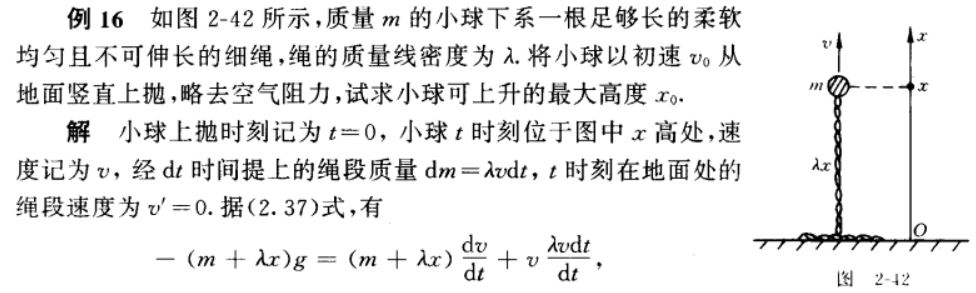
\includegraphics[width=.8\linewidth]{fig/力学题.JPG}
      \caption{密歇尔斯基方程应用题}
      \label{fig:mechanics}
    \end{figure}
    
    如上所述,利用密歇尔斯基方程重要的是确定主体是什么,这里主体是已经离地处于空中的绳子,而即将加入主体的部分是仍然“躺在”地上的一短节绳子。由于这时“躺在”地上的一节绳子是软的,对主体没有力的作用,因此主体受力只有重力,由此可列出上面的方程.原则上本题的物理部分就结束了,接下来是复杂的数学求解,结果为:
  
    \begin{equation*}
    (m + \lambda x)^{2}v^{2} = - \frac{2g}{3\lambda}(m + \lambda x)^{3} + \frac{2g}{3\lambda}m^{3} + m^{2}v_{0}^{2}
    \end{equation*}

    \begin{equation*}
    x_{0} = \frac{m}{\lambda}\left( \sqrt[3]{1 + \frac{3\lambda v_{0}^{2}}{2mg}} + 1 \right)
    \end{equation*}
    接下来又是物理的部分——通过考虑特殊情况检查结果的正确性:
    
    \begin{enumerate}[leftmargin=*, labelsep=0.5em]
      \item 如果绳子无质量,应当预期这时与直接抛掷一个小球得到的结果无差别,为$x_{0} = \frac{v_{0}^{2}}{2g}$.在上面的公式中令$\lambda \rightarrow 0$确实得到预期结果.
      \item 如果无外力,则显然$x_{0} \rightarrow \infty$.这时可以通过检查$v$的表达式,有$(m + \lambda x)v = mv_{0}$,这实际上就是动量守恒方程,小球和所有绳子构成的系统动量守恒,在初始时动量全部位于小球上,$p = mv_{0}$.随着绳子被拉动,动量分布于小球和被拉动的绳子上,$p = (m + \lambda x)v$.
      \item 一个有趣的问题是考虑$m \rightarrow 0$,计算结果给出这时$x_{0} \rightarrow 0$.这似乎与直觉有矛盾,$m \rightarrow 0$似乎意味着不在绳子前端挂一个小球而给绳端一个初速度将绳子拉起,为何会有$x_{0} \rightarrow 0$呢?仔细考虑会发现是我们的直觉错了,或者说我们弄错了物理图像——给绳端一个初速度将绳子拉起并不对应$m \rightarrow 0$的情况。当我们试图拉起一段绳子时,一定要有一段绳子已经被拉起来了,因为按照这个问题的假设,你只能对已经拉起来的部分施加力而无法对盘绕在地下的软绳下手。绳子前面挂的小球实际上可以理解为最初已经被拉起来的绳端,如果根本就没有绳端,即$m \rightarrow 0$,那显然无法将绳子拉起,即$x_{0} \rightarrow 0$.按照上面的考虑也能理解——当$m \rightarrow 0$时我们根本就没有为这个系统输入初始的动量,自然无法使绳子升起.
    \end{enumerate}
    
    简单总结一下,在做一个题目时,通常分为三个阶段:
    
    \begin{enumerate}[leftmargin=*, labelsep=0.5em]
      \item 物理的部分:理解题目所给出的物理情景,将其转化为数学方程
      \item 数学的部分:求解方程(这往往是大多数人关注的地方,但这其实是最不重要的地方)
      \item 物理的部分:对结果进行“反思”,能否给出其正确的证据?结果是否与直觉符合,如果不符合那么是结果错了还是直觉错了?得出结果后的“反思”十分重要,杨振宁在清华教授普通物理时曾谈到过:“在学习的过程中要重视直觉。当直觉与书本知识冲突时,是最好的学习机会,必须抓住这种时机,因为直觉不断被修正的过程就是自我提升的过程,直觉会带领我们走向新的研究领域。”(\url{https://www.bilibili.com/video/BV1194y1m73E/})
    \end{enumerate}
    
    \item 流体力学:流体力学的基本方程是Navier-Stokes方程
    
    \begin{equation*}
    \rho\left\lbrack \frac{\partial\mathbf{u}}{\partial t} + \left( \mathbf{u} \cdot \nabla \right)\mathbf{u} \right\rbrack\mathbf{= -}\nabla p + \eta\nabla^{2}\mathbf{u} + \rho\mathbf{g}
    \end{equation*}
    
    其中$\mathbf{u}$是流场中某点流体的速度,$\mathbf{g}$是单位体积受到的力,$\eta$是动力黏度描述液体的粘性。纯粹数学上看,这只是一个偏微分方程,那么一个学习物理的人会如何理解这个方程呢?
    
    \begin{enumerate}[leftmargin=*, labelsep=0.5em]
      \item 它实际上是流体中一个体元的牛顿运动定律,左侧的项(随体导数项)$\frac{D\mathbf{u}}{dt} = \frac{\partial\mathbf{u}}{\partial t} + \left( \mathbf{u} \cdot \nabla \right)\mathbf{u}$实际上给出了跟随流体中的一个微元运动时的加速度而右侧的项即其受力。随体导数项当然可以通过链式求导法则进行对欧拉描述和拉格朗日描述之间的转换得到,但正如上面说的,看到一个公式最重要的是通过考虑特殊情况使自己相信这时正确的。不妨考虑一维情况,则该项为$\frac{Du}{dt} = \frac{\partial u}{\partial t} + u\frac{\partial u}{\partial x}$.
      
      \begin{figure}[H]
        \centering
        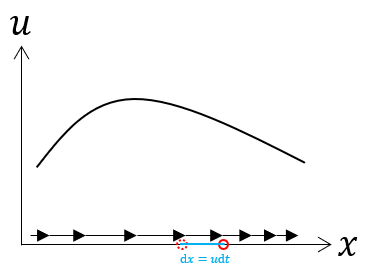
\includegraphics[width=.35\linewidth]{fig/速度场.png}
        \caption{随体导数示意图}
        \label{fig:derivative}
      \end{figure}
        
      不妨考虑恒定速度场则只需关注第二项,在一个很短的时间内,微元从原先的位置$x$(图中虚线)运动到新的位置$x + dx$(图中实线),进而也获得了新的速度$u(x + dx)$.在该过程中速度变化为$du = u(x + dx) - u(x) = \frac{\partial u}{\partial x} \cdot dx = \frac{\partial u}{\partial x}udt$,于是加速度为$a = \frac{du}{dt} = u\frac{\partial u}{\partial x}$.当然这实际上就等同于使用链式法则进行计算,但通过这种方式更容易看出数学表达式背后的物理过程。
      
      \item 它包含了流体中最重要的两个效应——惯性和黏性,惯性与质量有关,因此表述惯性的项是左侧的$\rho\left\lbrack \frac{\partial\mathbf{u}}{\partial t} + \left( \mathbf{u} \cdot \nabla \right)\mathbf{u} \right\rbrack$,而表述黏性的项即$\eta\nabla^{2}\mathbf{u}$.当惯性主导时,即$\rho \rightarrow \infty$,方程变为$\frac{D\mathbf{u}}{dt} = \frac{\partial\mathbf{u}}{\partial t} + \left( \mathbf{u} \cdot \nabla \right)\mathbf{u}$,这是我们非常熟悉的方程,它实际上就描述了流体中的微元的自由运动;当粘性主导时,即$\eta \rightarrow \infty\ $,方程变为$\nabla^{2}\mathbf{u} = 0$,经过热学课程的学习就能看出,这实际上就是扩散方程,描述了流体中粒子的扩散,黏性来源于粒子扩散。上面做的这些把方程的项与物理因素联系了起来。这有什么用呢?经验告诉我们,非线性的问题是复杂的而线性的问题通常是简单的,流体中非线性造成的复杂现象是湍流。方程中的速度非线性项是$\left( \mathbf{u} \cdot \nabla \right)\mathbf{u}$,它是惯性效应的一部分,因此我们知道,当惯性效应较强时,会存在复杂的湍流现象,而反之当粘性效应较强时,流动会较为规整。这是符合我们的直觉的,当我们倒出蜂蜜、挤出牙膏时,从未见过湍流的产生,但在奔涌的江河中却随处可见湍流。此外,我们知道非线性项$\left( \mathbf{u} \cdot \nabla \right)\mathbf{u}$的强度取决于速度的大小和速度变化的空间尺度$L$,当$u$本身很小时,非线性项的大小是$u^{2}$量级,与$u$相比可以忽略,另一方面若$u$根本无空间变化,该非线性项也不存在。因此决定湍流产生的参量应该与$u,\ L,\ \rho,\ \eta$有关,结合上面的直觉,该参量与$\rho$和$\eta$的相关关系应当相反,结合量纲分析能够确定唯一的参量:
      
      \[Re = \frac{\rho vL}{\eta}\]
      
      这就是雷诺数,在上面的分析中我们没有用到任何的数学推导,完全凭借对公式中各个项的物理图像的分析和物理直觉。
    \end{enumerate}
\end{enumerate}
\end{myexample}

怎样重视物理图像?答案其实就在上面的文字中:

\begin{enumerate}[leftmargin=*, labelsep=0.5em]
\item 在日常的学习中,每当接触到一个新的方程,按照上面例子中的方式,\textbf{关注每个物理量的内涵,思考方程中每一项对应的物理过程,尝试将方程变为直觉(找出它是对的证据)。}

\item 在完成习题时,不应当只关注数学运算。\textbf{列出数学表达式前应弄清物理过程(最好画出几张图),在得出结果时停下来“反思”,试图说明结果的正确性,思考结果与直觉是否符合。}
\end{enumerate}

\addcontentsline{toc}{subsection}{问题五:初学物理课程时,怎样适应物理课使用高等数学方法解决问题的思路?}
\noindent$\blacktriangleright$\;\textbf{Q5:} 初学物理课程时,怎样适应物理课\textbf{使用高等数学方法解决问题}的思路?

\noindent$\blacktriangleright$\;\textbf{A5:}

据我观察,许多大一的同学发现自己力学、热学不会做题、学不明白,实际上不是没有理解物理概念,而是没有适应使用高等数学方法解决问题。许多物理问题的分析利用了“微元法”,即考虑微过程或者物体微元,列出微分方程并求解。或者是先假设未知的物理量,结合各种条件列出代数方程组并联立求解(可能有人会认为这是十分自然的,但从我接触到的同学来看,这并不十分自然。实际上这个过程需要很复杂的总揽全局的思维,需要始终关注\textbf{有哪些未知量?已经列出了哪些方程?还需要或者可能列出哪些方程?某个未知量通常会以什么方式出现在方程中?}这实际上是需要通过训练才能具有的能力)。一方面,国科大的数学教育过于重视证明而轻视应用,导致许多同学不具备相应的数学能力;另一方面,高中物理通常都是一个式子得出一个结果,很少有需要列出大量方程联立求解或者分析微元得出微分方程的问题,同学们往往不适应这些思维方式。解决方案也很简单,首先需要认识到问题,当你有很多题目不会做,但仔细分析发现都是不懂得使用上面提到的基本的数学思想时,不要慌张你并不是没有学会物理概念,缺乏的只是对数学思想的练习——“无他,惟手熟尔”!

首先你需要有基本的数学知识,建议仔细通读舒幼生《力学》的数学附录,做到对基本积分的计算、泰勒公式及其应用、导出及求解微分方程和代数方程十分熟悉(其他的参考书如李忠《高等数学》或者《普林斯顿微积分读本》)。其次需要对上面提到的几种基本的数学思想(\textbf{微元分析}、\textbf{对多个待定未知量列出联立方程求解})有印象,可以将平时遇到的没有做出来的题目记下来(没有必要用诸如“错题本”、“考点整理本”之类的繁复没用的东西,只要能让自己有印象就行),进行简单归纳——哪些情况下可能会使用微元分析的方法?什么时候需要引进新的未知数并联立方程求解?

最后,上面说到的这些数学方法仅仅是冰山一角,一个成熟的科学工作者往往有独属于自己的一套“工具箱”,里面有许多自己用的十分熟练的“工具”。我的个人经验是,当遇到一个习题无法解决时,我会果断看答案而不是与它死磕,如果答案使用的方法在我的工具箱内,那么我会想\textbf{为什么会想到使用这个方法?之前我遇见过类似的问题吗?能否为这个方法建立一个相对固定的对应?}(例如:是不是存在某个条件的问题都可以使用这个方法?这种方法是否可以进行推广以适用于更多类似的问题?)如果答案使用的方法不在我的工具箱内,那么我会首先尝试\textbf{重新使用我工具箱内的方法解决这个问题}(与没有看到答案不同,答案能够提供给我对问题更多的洞察),如果不能那么\textbf{我仅有的方法能够将这个问题解决到哪一步?它们分别具有什么瓶颈?应该怎样修改这个问题使得我可以用我已有的方法解决?这个新的方法是否可以推广成为一个普适性的工具还是仅仅是对于某个问题的巧合?}如果是前者,那么恭喜我们的工具箱中有多了一件工具!

上面说的这些不局限于物理题目,对于数学证明/求解题目同样适用,甚至对于各种学科中的科研问题,也是一样的。

\begin{myexample}
  举一个例子,这个问题可能已经进入了许多省市的高中物理教学中,但我相信许多人没能深刻理解它。  
  
  考虑一个带电量为$q$,质量为$m$的粒子在垂直纸面的磁场和重力场的叠加场中的运动,初始速度为$\mathbf{v}_{0}$(见下图),求其后续的运动。
  
  \begin{figure}[H]
    \centering
    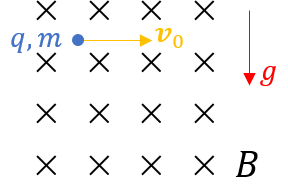
\includegraphics[width=.3\linewidth]{fig/配速.png}
    \caption{带电粒子在磁场和重力场中的运动}
    \label{fig:particle_motion}
  \end{figure}
  
  据我所知,在一些省市的高中物理教学中,该问题通常会使用一种被称为“配速法”的方式求解,其操作步骤可以用下图概括:
  
  \begin{figure}[H]
    \centering
    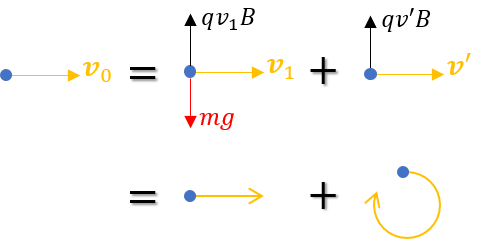
\includegraphics[width=.4\linewidth]{fig/配速运动.png}
    \caption{配速法的操作步骤}
    \label{fig:method}
  \end{figure}
  
  将初始速度$v_{0}$分解为$v_{1} + v'$,其中$v_{1} = \frac{mg}{qB}$用于“消去”重力,对应于一个不受外力的匀速直线运动,而$v'$对应的运动仅受到磁场,对应于一个匀速圆周运动,物体的运动就是匀速直线运动和匀速圆周运动的叠加。
  
  这个求解问题的方式十分精妙,可是在看过这个方法之后呢?绝大部分学习者都只是记住了操作方式但没有深挖一步——\textbf{为什么会想到这个方法?}
  
  对这个问题的回答可能有几种:
  
  \begin{enumerate}[leftmargin=*, labelsep=0.5em]
    \item “这是一个天才的想法,完全没有逻辑但就是能否解决这个问题”——这是对这种问题最浅层的回答,小心这种回答,因为大部分看起来十分天才的想法,都有更自然的逻辑,只是你没有找到或者没有足够高的视角。这种时候你只能先对这个方法有些印象,等到以后见到更多的例子或者学习到更深刻的结论再研究。
    
    \item “这是一个针对这种问题特殊的方法,它利用了问题的某种性质,\textbf{它可以进行推广},具有这种性质的问题通常都可以使用这种方法”——这比上面一层更深一步,它的好处是\textbf{我们将这种方法与问题的某种性质、某种特殊的条件联系起来},这使得我们建立一个对应,一旦见到这种条件往往可以用这种问题,\textbf{并且最重要的是我们意识到这种方法可以推广}。这时我们应该考虑,它能推广到什么程度?找到一些别的例子,这些例子有什么共性?从这些共性中能否总结出更本质地东西?
    
    对于这个问题,我们会发现如果磁场和重力场不垂直,也可以使用这种方法;可是如果外场不是恒定地重力场而是空间分布不均匀的电场似乎就不能使用该方法;如果再进一步就会发现(或者通过接触更多的问题),我们实际上并没有用到磁场力与运动方向垂直的性质,将磁场力换成阻力$\mathbf{f} = - \gamma\mathbf{v}$也可以使用一模一样的方法。结合上面这些可以使用和不可以使用的情况我们可以总结出,在存在任何恒定的力场和磁场力或阻力时,无论两种力之间呈现什么关系,都可以使用配速法。这已经比第一种回答更进一步了,但还可以更进一步思考,磁场力$\mathbf{F} = q\mathbf{v} \times \mathbf{B}$与阻力$\mathbf{f} = - \gamma\mathbf{v}$之间有什么共性?这就引发我们走向第三层
    
    
    \item “这本质上是某种\textbf{普适的思想或者方法在特殊问题上的应用}”——这是最深层的回答,但它不是直接就能达到的,需要见到大量的例子并把它们放在一起思考才能看出。
    
    对于这个问题,我们会发现,$\mathbf{F} = q\mathbf{v} \times \mathbf{B}$
    与$\mathbf{f} = - \gamma\mathbf{v}$的共性就是它们都是线性的。为了更清楚地看到配速法的本质,我们将这个问题一般性地写为求解方程
    
    \begin{equation*}
    m\ \ddot{\mathbf{r}} = q\ \dot{\mathbf{r}} \times \mathbf{B} + m\mathbf{g}
    \end{equation*}
    
    我们刚才所作的实际上是将解$\mathbf{r}(t)$写为$\mathbf{r}(t) = \mathbf{r}^{\mathbf{'}}(t) + \mathbf{v}_{1}t$,带入方程就得到:
    
    \begin{equation*}
    m\ddot{\mathbf{r}^{\mathbf{'}}} = q\left( \dot{\mathbf{r}^{\mathbf{'}}} + \mathbf{v}_{1} \right) \times \mathbf{B} + m\mathbf{g} \Longrightarrow m\ddot{\mathbf{r}^{\mathbf{'}}} = q\dot{\mathbf{r}^{\mathbf{'}}} \times \mathbf{B} + \cancel{\left( q\mathbf{v}_{1}\mathbf{\times B} + m\mathbf{g} \right)}
    \end{equation*}
    
    则剩下的只是:
    
    \begin{equation*}
    m\ddot{\mathbf{r}^{\mathbf{'}}} = q\dot{\mathbf{r}^{\mathbf{'}}} \times \mathbf{B}
    \end{equation*}
    
    这也就是我们说两种运动可以独立叠加的逻辑。回忆在微积分中学到的,便会发现这种方法是相当一般的,我们在解非齐次线性微分方程时,基本的思想就是将其写为齐次通解和非齐次特解的组合,而配速法,虽然外观上伪装成一种巧妙的构造,但实际上就是线性问题齐次化的思想。
    
    可能我们都会解诸如$\ddot{x} + 3\dot{x} + 2x = \cos{3t}$这样的方程,但有没有意识到,这个问题与看起来毫无关系的配速法本质上是一样的?当然,上面说的这些可能我们在最开始时并不能走那么深,但从现在开始尝试,在做完一道题时深入地想一想,最终也能达到举一反三的境界!
  \end{enumerate}
    
  仍然是这个问题,常见的还有另一种方法(例如见朗道《场论》),考虑在$xy$平面中列出两个联立方程:
  
  \begin{equation*}
    \left\{
  \begin{aligned}
  m\ddot{x} &= -q\dot{y}B \\
  m\ddot{y} &= q\dot{x}B - mg
  \end{aligned}\right.
  \end{equation*}
  
  这时考虑令$\zeta = x + iy$则得到:
  
  \begin{equation*}
  m\ddot{\zeta} = iqB\dot{\zeta} - img
  \end{equation*}
  
  这时只需要求解这种单复变量的方程就可以了。和上面一样,我们能否对着它思考一会儿?这种借助复数的方法可以推广吗?什么情况下考虑复数会更简便?还有别的利用复数简化问题的例子吗?它们有什么共性?这些问题留给正在阅读本文的你!
\end{myexample}
  
\addcontentsline{toc}{subsection}{问题六:一些复杂的证明或者公式推导根本记不住但有时期末还要考,学完就忘怎么办?}
\noindent$\blacktriangleright$\;\textbf{Q6:}一些复杂的证明或者公式推导根本记不住但有时期末还要考,\textbf{学完就忘}怎么办?
  
\noindent$\blacktriangleright$\;\textbf{A6:}

首先,这十分正常!除非在接下来的学习或工作中反复用到某些结果,否则你在学完后几乎肯定会忘掉已经学过的各种结果。学习更加重要的是,对这个结果有一个大致的印象,在需要用到时知道应该从哪里找到这个结果或者能够在脑中仅有的印象的指导下推导出这个结果。

要做到这一点,关键仍然是上面说的,对一个公式/定理存在一个粗略的、感觉性的认识,对其证明的大体框架、每一步在干什么有印象(而不是记住各种细节)。在学完一个定理或者证明之后,问问自己,\textbf{我能否用一句非常简单的话就概括出它在讲一件什么事?}

\begin{myexample}
  
举一个例子,我们看“线性代数基本定理”:
  
  \begin{quote}
    对于线性映射$\mathcal{A}:V \rightarrow W$,有$\dim{\ker\mathcal{A}} + \dim{\operatorname{Im} \mathcal{A}} = \dim V$(对于矩阵$M_{n \times m}$,有类似的版本:$\operatorname{rank} M + \operatorname{null} M = m$)
  \end{quote}
  
  该定理涉及三个概念,每个概念理解起来都花费一定时间,将三个加起来就更加容易忘记。为了加深对它的印象,仍然尝试举出一些特殊情况来使自己相信这个定理是对的,获得对它的直觉。
  
  设想$\mathcal{A}$是一个简单的嵌入映射,比如把一个二维平面嵌入到三维空间中,即$\mathcal{A}: \mathbb{R}^{2} \rightarrow \mathbb{R}^{3}$,那么这时核空间维数是0,而象空间实际上就是$\mathbb{R}^{3}$中的二维子空间(即对应的二维平面),这时等式显然成立,实际上只要考虑到这个例子就不会把公式的右侧记错成$\dim W$.再次考虑$\mathcal{A}: \mathbb{R}^{3} \rightarrow \mathbb{R}^{3}$是一个把三维空间中第三个维度压缩掉并将前两个维度进行一定的扭曲的映射(例如:$(x,y,z)\overset{\mathcal{A}}{\mapsto}(2x + y, - y,0)$),那么这时象空间即$\mathbb{R}^{3}$中的$xy$平面,而核空间即被压缩掉的第三个维度对应的空间,等式也是成立的。看完几个例子,我们能否用直觉性的表述来把这个定理讲出来?看第二个例子,直观上,$\mathcal{A}$似乎将原有的空间$V$分成两部分,一部分是其没有“压缩”保持完好的部分(其中的$xy$平面),在经过一定的扭曲之后被变换为象$\operatorname{Im} \mathcal{A}$,原先没有被“压缩”的部分有多么大的自由活动程度,在被变换后仍然有多么大的自由度,不会因此变得更大。而另一部分是“压缩掉”的部分,也就是$\ker\mathcal{A}$.这样一看,线性代数基本定理实际上就是上面这个“将原有的空间$V$分成两部分”的直观说法的精确描述。这种直观还能启发我们想到这个定理的证明(读者自己试一试)
\end{myexample}
  
\addcontentsline{toc}{subsection}{问题七:上课大部分都听不懂怎么办?}
\noindent$\blacktriangleright$\;\textbf{Q7:} 上课大部分都听不懂怎么办?
  
\noindent$\blacktriangleright$\;\textbf{A7:}
  
不用担心,这很正常!学习一门课最核心的目标就是掌握知识,在知识相同的情况下,有许多种理解、串联、讲授知识的方法,每个人都有自己适合的理解知识的方式和节奏,适合自己的才是最好的,上课听不懂不一定是自己的问题,可能只是老师讲授的方式与节奏不适合自己。

想想自己为什么听不懂,是老师讲解的节奏太快、引入概念的方式晦涩抽象?还是自己先前的知识掌握不熟练跟不上?如果是后者,那么首要的是抽出时间将前面的内容掌握明白(以及还要知道,正常来说听课的时候有少部分内容跟不上是很正常的,只要能够理解整体框架就算是听懂了)。但如果是前者,那么完全可以尝试以自学为主、听课为辅的方式。自学的好处是能够按照自己的节奏学习知识,可以不完全按照讲课的逻辑学习(例如,对于同一个定理,如果讲课时讲授的证明方法无法理解,只要能够找到让自己理解定理的方式就可以,不用一定强求自己看懂讲课时讲授的方法)——只要能够让自己学懂,任何方法都是可以的。

笔者自认为很笨,很多时候一个概念身边人很快理解了我还没能搞懂,上课经常跟不上很多时候完全听不懂,课下自己会去反复琢磨,因此形成了自学为主的习惯。在这里我也向有同样问题的人说一句:我这么笨的人都能够自己一点点把很复杂的东西搞懂,你也肯定可以!

\noindent$\blacktriangleright$\;其他话题:

\begin{enumerate}[leftmargin=*, labelsep=0.5em]
\item 一些不错的\textbf{学习资源}

一些参考书:

\begin{itemize}
  \item 微积分/数学分析:\textbf{谢慧民《数学分析习题课讲义》}(这本书里每一节都有很细致的方法和例题的讲解以及概念辨析,可以借此深入对于定理和方法的理解,十分推荐!)以及与之类似的裴礼文《数学分析中的典型问题与方法》、菲赫金哥尔茨《微积分学教程》(很厚的书,有很多计算的例子)
  
    \item 线性代数:\textbf{丘维生《高等代数》}(很厚的书,讲解十分细致,有大量有答案的例题,内容几乎覆盖了国科大线性代数课的全部内容,B站上有作者自己的授课视频)、\textbf{Sheldon Alex \textit{Linear Algebra Done Right}}(中译本《线性代数应该这样学》,与线性代数II的内容重合很多但讲解更清晰)、李尚志《线性代数学习指导》(有大量的有答案的例题和方法讲解)、3Blue1Brown “线性代数的本质”系列视频(B站:\url{https://www.bilibili.com/video/BV1ys411472E} 有许多对概念直观的解释)、蓝以中《高等代数简明教程》(虽然简明但对概念和逻辑的讲解十分清晰)
  
  \item 力学:指定参考书舒幼生《力学》就很不错,除此之外很不错的参考书是丹尼尔·克莱普纳《力学概论》,有大量例子,许多有具体的科研情景,讲解也十分细致,内容比舒幼生《力学》略多。
\end{itemize}

一些网站推荐:

\begin{itemize}
  \item 英文论坛,看书时不懂的问题能够在这里获得十分专业的回答
  
  Physics Stack Exchange(\url{https://physics.stackexchange.com/})
  
  Mathematics Stack Exchange(\url{https://math.stackexchange.com/})
  
  \item 知乎:不要笑,知乎真的是一个学习软件!能够从中找到许多的经验分享、书籍推荐、复习总结以及对某些问题的探讨。
\end{itemize}

\item \textbf{如何提问}

\begin{itemize}
\item \textbf{提问时应当展示自己的思考与努力。}例如与其问“这个问题我不会,应该怎么做?”不如问“我尝试了某些方法,但它们卡住了,我认为这个问题可能从这些角度突破但我没有头绪,应该怎么做?”,回答者可以有针对性地针对你的尝试回答问题,分析你为什么没能成功。

\item \textbf{提问应当具体,最好有一些实际例子。}例如与其问“我这门课学不会,应该怎么学?”不如问“我对某一章的概念没有理解好,能否帮忙梳理这一章的内容?”、“我掌握了章节的重要内容,但是课后习题,比如这些题不会做,应该怎样加深对知识的掌握以达到熟练解决问题的水平”。与其问“我考试考得很差,应该怎么办?”不如问“考试的时候我这几道题做错了,当时我是怎么想的,能否帮忙分析一下原因?”

\item \textbf{尽量问“授人以渔”的问题而不是问“授人以鱼”的问题。}例如与其问“这个题怎么做?”不如问“这几道相同类型的题有什么共性的方法?”
\end{itemize}
\end{enumerate}

\section{结语}
\begin{center}
  \kaishu 谨以此文献给陪伴我多年的老猫、我的父母和在我写作此文时给予我无限灵感的可爱的同学们!
\end{center}

现在看我在序中写下的文字,还能回忆起那天的几乎全部细节,那半年前的一天仿佛就在昨天。在这过去的半年里,我经历了太多曲曲折折的大事件,而这篇文章我几乎是放弃了。原因无他,仍然是担心就算我费尽心思写完这篇满是废话文章,它又能帮到多少人呢?差不多是半个月前,我又拾起了续写此文的热情,将几乎快完工的文稿上传到网络上,又将其送予一些挚友审阅批判,没想到的是,在短短几天里我收到了许多正面的评价,这给予我极大的信心并在接下来的几天内将文章仔细修改完善。在此我向那些忍受我长篇废话并给予我鼓励的同学和网友致以最诚挚的感谢!

我知道或许我的这篇文章会被误解为“鼓励新生内卷”而遭批判,或许我就此将这篇文章删除对我而言更好。思虑许久我选择发声而不是沉默——在高中时我学习物理竞赛,由于赛前复习阶段没有教练,且我又是全年级仅剩唯一的物理竞赛生,在遇到问题时无法请教,只能自己窝在实验室的一角一边反复思索一边查阅着各种资料,这种时刻我无比渴望有一个已经“趟水过河”了的学长能够在一旁解答我的困惑。这段经历让我格外在意他人的提问,因为那一个个提问题的人总让我想起高中时的我,我理解百思不得其解的痛苦和对一个满意的解答的渴望。虽然进入大学时,由于有竞赛基础在学习数理基础课方面相对轻松,但我能切身感受到数理基础课程为许多同学带来的痛苦——我想为正被数理基础所折磨的同学们发声。我喜欢罗素的那句话:
\begin{quotation}
  Three passions, simple but overwhelmingly strong, have governed my life: the longing for love, the search for knowledge, and unbearable pity for the suffering of mankind.
\end{quotation}
我为我现在还能保有“对苦难的怜悯”而感到自豪!

希望这篇文章能够帮助到对“如何学好数理基础课”这一问题而感到困惑的大一同学!

{\hfill 2025年7月28日\quad 于山东大学洪家楼校区\;济南振声学校\;励学楼}
\end{document}
